\pdfminorversion=7%
\documentclass[aspectratio=169,mathserif,notheorems]{beamer}%
%
\xdef\bookbaseDir{../../bookbase}%
\xdef\sharedDir{../../shared}%
\RequirePackage{\bookbaseDir/styles/slides}%
\RequirePackage{\sharedDir/styles/styles}%
\toggleToGerman%
%
\subtitle{16.~Gleichheit und Identität}%
%
\begin{document}%
%
\startPresentation%
%
\section{Einleitung}%
%%
\begin{frame}%
\frametitle{Einleitung}%
\begin{itemize}%
\item Wir benutzen Variablen, um Objekte im Speicher zu referenzieren.%
\item<2-> Wenn wir zwei Variablen vergleichen, dann vergleichen wir genau genommen die Ojekte, die sie referenzieren.%
\item<3-> Es ist klar, dass zwei Variablen auf Objekte verweisen können, die \emph{gleich} oder \emph{ungleich} seien können.%
\item<4-> Sie können aber auch das \emph{selbe Objekt} referenzieren.%
\item<5-> Wir müssen diese beiden Konzepte, \emph{Gleichheit} und \emph{Identität}, unterscheiden.%
\end{itemize}%
\end{frame}%
%
\section{Gleichheit und Identität}%
%
\begin{frame}%
\frametitle{Gleichheit und Identität}%
\begin{itemize}%
\item Wir müssen diese beiden Konzepte, \emph{Gleichheit} und \emph{Identität}, unterscheiden.%
\item<2-> Und das ist einfach.%
%
\item<3-> Stellen Sie sich vor, dass Sie eine grüne Jacke kaufen. Wir nennen sie~$A$.%
%
\item<4-> Am nächsten Tag kaufen Sie eine gleiche güne Jacke. Wie nennen sie~$B$.%
%
\item<5-> Nun haben Sie zwei \emph{gleiche} Jacken, $A$ und $B$. Es gilt \pythonil{A == B}.%
%
\item<6-> $A$ und $B$ sind Namen für zwei separate Objekte mit verschiedener Identität. Es gilt~\pythonil{A is not B}.%
%
\item<7-> Sie können Jacke~$A$ in den Kleiderschrank tun. Wenn Sie sie morgen herausholen, können Sie die Jacke~$C$ nennen.%
%
\item<8-> Dann sind $A$ und $C$ zwei Namen für ein und das selbe Objekt. Es gilt \pythonil{A == C} und \pythonil{A is C}.%
%
\end{itemize}%
\end{frame}%
%
\begin{frame}[b]%
\frametitle{Gleichheit und Identität Illustriert}%
%
\locate{}{\resizebox{0.8\paperwidth}{!}{%
%
\begin{tabular}{r@{:~}lr@{:~}lr@{:~}l}%
\multicolumn{2}{c}{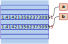
\includegraphics[width=0.275\paperwidth]{graphics/different}}&%
\multicolumn{2}{c}{\uncover<2->{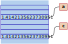
\includegraphics[width=0.275\paperwidth]{graphics/equal}}}&%
\multicolumn{2}{c}{\uncover<4->{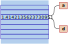
\includegraphics[width=0.275\paperwidth]{graphics/same}}}\\%
%
\pythonil{a == b}&\pythonil{False}&%
\uncover<2->{\pythonil{a == c}}&\uncover<2->{\pythonil{True}}&%
\uncover<4->{\pythonil{a == d}}&\uncover<4->{\pythonil{True}}\\%
%
\pythonil{a is b}&\pythonil{False}&%
\uncover<2->{\pythonil{a is c}}&\uncover<2->{\pythonil{False}}&%
\uncover<4->{\pythonil{a is d}}&\uncover<4->{\pythonil{True}}\\%
\end{tabular}%
%
}}{0.1}{0.13}%
%
\begin{itemize}%
%
\item Wenn wir zwei Variablen \pythonil{a=1.4142135623730951} und \pythonil{b=1.4142135623730953} haben, dann referenzieren sie verschiedene Objekte mit verschiednen \pythonil{float}-Werten, die an verschiedenen Speicherstellen stehen.%
%
\item<2-> Jetzt haben wir eine dritte Variable~\pythonil{c}, die ein \pythonil{float}-Object referenziert, dass den gleichen Wert wie~\pythonil{a} speichert.%
\item<3-> Weil es ein anderes Objekt ist, steht es auch woanders im Speicher.%
%
\item<4-> Setzen wir \pythonil{d = a}, dann zeigt \pythonil{d} auf das selbe (identische) \pythonil{float}-Object wie~\pythonil{a}, auf die selbe Speicherstelle.%
%
\end{itemize}%
%
\end{frame}%
%
\begin{frame}%
\frametitle{Beispiel~1}%
%
\gitLoadAndExecPython{variables:identity_1}{}{variables}{identity_1.py}{}%
\listingPythonAndOutput{}{variables:identity_1}{}{0.05}{0.086}{0.9}{0.92}%
%
\end{frame}%
%
\begin{frame}%
\frametitle{Beispiel~2}%
%
\parbox{0.334\paperwidth}{\small{%%
\begin{itemize}%
\item String-\glslink{literal}{Literale} werden gecached und wiederverwendet, Verbindungen von String-Literalen in einem Ausdruck werden gleich als String-Literale interpretiert -- \pythonil{a}, \pythonil{b}, und \pythonil{c} sind das selbe Objekt.%
\item<2-> \pythonil{d} wird in zwei Schritten berechnet, kommt nicht aus dem Cache, und ist daher ein anderes Objekt.%
\item<3-> Implementationsspezifisch cached und wiederverwendet der \python-Interpreter kleine Integer-Werte~(\pythonil{e} und \pythonil{f}).%
\item<4-> Große aber nicht~(\pythonil{g} und~\pythonil{h}).%
\end{itemize}%
}}%
%
\gitLoadAndExecPython{variables:identity_2}{}{variables}{identity_2.py}{}%
\listingPythonAndOutput{}{variables:identity_2}{}{0.395}{0.05}{0.9}{0.92}%
\end{frame}%
%
\section{Zusammenfassung}%
%
\begin{frame}%
\frametitle{Zusammenfassung}%
\begin{itemize}%
\item Wir unterscheiden \emph{Gleichheit} und \emph{Identität}.%
\item<2-> Gleichheit wird mit dem Operator~\pythonil{==} und Ungleichheit mit~\pythonil{!=} geprüft.%
\item<3-> Identität wird mit dem Operator~\pythonil{is} und nicht-Identität mit~\pythonil{is not} geprüft.%
\item<4-> Zwei separate Objekte können gleich oder ungleich sein, aber niemals identisch.%
\item<5-> Zwei identische Objekte sind immer gleich, also \pythonil{A is B}$\Rightarrow$\pythonil{A == B}.%
\end{itemize}%
\end{frame}%
%
\endPresentation%
\end{document}%%
\endinput%
%
